\section{AMR-Based Detonation Solver in OpenFOAM}

\begin{frame}{OpenFOAM Overview}
\begin{itemize}
\item Open-source, free, computational fluid dynamics toolbox 
\item Written in C++, has many solvers 
\item No GUI, file-based input and control
\end{itemize}
\end{frame}

\begin{frame}{Tested Solvers}
Solvers tested for their capability to model shocks and detonations:
\begin{itemize}
\item \textbf{rhoReactingFoam}: included with OpenFOAM, a density-based combustion solver
\item \textbf{rhoCentralFoam}: included with OpenFOAM and developed by Greenshields \textit{et. al.} \cite{greenshields}, a density-based solver that uses the central-upwind schemes of Kurganov and Tadmor \cite{kurganov1} 
\item \textbf{rhoReactingCentralFoam}: a solver combined by Caelan Lapointe with previous work done by Nakul \cite{nakul}, with AMR support
\end{itemize}
\end{frame}

\begin{frame}[allowframebreaks]{Governing Equations}
Detonations were modeled using the reacting Navier-Stokes equations \cite{kuo,stokes}:
\begin{equation}
\frac{\partial \rho}{\partial t} + \nabla \cdot \left(\rho \bm{u}\right) = 0\,
\end{equation}
\begin{equation}
\frac{\partial \rho\bm{u}}{\partial t} + \nabla \cdot \left(\rho \bm{u}\otimes \bm{u}\right) + \nabla p -\mu\nabla^2\bm{u}= \bm{0}\,,
\end{equation}
\begin{equation}
\frac{\partial \rho E}{\partial t} + \nabla \cdot \left[\left(\rho E + p\right)\bm{u}\right] -\alpha\nabla^2 e = \dot{q}\,,
\end{equation}
\begin{equation}
\frac{\partial \rho Y_i}{\partial t} + \nabla \cdot \left(\rho Y_i \bm{u}\right) -\mu\nabla^2 Y_i= \dot{\omega}_i\,,
\end{equation}
where 
\begin{equation}
\dot{q} = \sum_{i = 1}^N \dot{\omega_i} \Delta h_{f,i}^0\,,
\end{equation}
%is the heat flux, $\dot{\omega}_i$ is the species source reaction rate, $\rho$ is the density, $\bm{u}$ is the fluid velocity vector, $Y_i$ is the mass fraction of the $i$th species, $E$ is the total energy, $p$ is the pressure, $\mu$ is the dynamic viscosity, $e$ is the internal energy, $\alpha$ is the thermal diffusivity and $\Delta h_{f,i}^0$ is the species formation enthalpy.

Total energy \cite{kuo} can be written as 
\begin{equation}
E = h - \frac{p}{\rho} +\frac{1}{2} \left(\bm{u}\cdot\bm{u}\right)\,,
\end{equation}
where the total summed enthalpy is written \cite{kuo} as 
\begin{equation}
h = \sum_{i = 1}^Nh_{s,i}Y_i\,,
\end{equation}
and the species total enthalpy \cite{kuo} is given by 
\begin{equation}
h_{i} = \Delta h_{f,i}^0 + h_{s,i}\,,
\end{equation}
with the sensible enthalpy for the $i$th species expressed as
\begin{equation}
h_{s,i} = \int_{T_0}^T C_{p,i}\mathrm{d}T\,,
\end{equation}
Here $C_{p,i}$ is the specific heat for the $i$th species, $T$ is the temperature, and $T_0$ is an initial, or reference, temperature. The equation of state is expressed as 
\begin{equation}
p = \rho R T\,,
\end{equation}
where $R=R_u/W$. Specific heat $C_{p,i}=C_{p,i}(T)$ from NIST JANAF \cite{janaf} lookup tables.  
\end{frame}

\begin{frame}{Notes About Governing Equations}
\begin{itemize}
\item No turbulence modeling 
\begin{itemize}
    \item subgrid-scale turbulence structures averaged out numerically
    \item akin to implicit LES
\end{itemize}
\item Not modeling inviscid Euler equations; viscosity is accounted for with Sutherland \cite{sutherland} model:
\end{itemize}
\begin{equation}
\mu = \frac{A_s \sqrt{T_s}}{1 + \frac{T_s}{T}} \,,
\end{equation}
\end{frame}

\begin{frame}{Chemical Reactions}
Single-step stoichiometric hydrogen-air utilized here, which follows the following expression \cite{kuo}:
\begin{center}
\ch{2 H2 + 2 (O2 + 3.76 N2) -> 2 H2O + 7.52 N2}
\end{center}
with
\begin{table}[t!]
\centering
\begin{tabular}{cc}
Species & Mass Fraction \\ \hline
H\(_2\) & 0.02851 \\ 
H\(_2\)O & 0 \\
N\(_2\) & 0.745 \\ 
O\(_2\) & 0.226 \\ \hline
Total & 0.99951 \\ 
\end{tabular}
\end{table}
\end{frame}

\begin{frame}{Reaction Rate Modeling}
Arrhenius equation \cite{arrhenius} takes the form \cite{christ} 
\begin{equation}
\dot{\omega}_i = AT^\beta \exp\left(\frac{E_a}{R T}\right)\,,
\end{equation}
where $Ta = Ea/R$. Simulation values were explored, but we settled on 
\begin{equation}
   A = 1.4 \times 10^{13} ~ \text{m}^3\text{mol}^{-1}\text{s}^{-1},
   \qquad 
   Ta = 12996 ~\text{K},
   \qquad
   \beta = 0\,.
\end{equation}
with \(R = 368.9\) J/Kg-K. As shown later these reasonably match Chapman-Jouguet detonation theory \cite{chapman} along with other published values \cite{towery1,hashemi}.
\end{frame}


\begin{frame}{OpenFOAM Finite Volume Numerical Schemes}
\begin{table}[t!]
\centering
%\caption{OpenFOAM finite volume numerical schemes applied during solving}
%\label{tab:numschemes}
\scalebox{0.9}{
\begin{tabular}{ccc}
Term & OpenFOAM Variable & Numerical Scheme \\ \hline 
Flux Scheme & \texttt{fluxScheme} & Kurganov \\ 
Time Scheme & \texttt{ddtSchemes} & Euler \\
Gradient Schemes & \texttt{gradSchemes} & Gauss linear \\ 
Divergence Schemes & \texttt{divSchemes} & none by default \\ 
& \texttt{div(tauMC)} & linear \\ 
& \texttt{div(phi,}specie\texttt{)} & van Leer \\ 
Laplacian Schemes & \texttt{laplacianSchemes} & Gauss linear uncorrected \\ 
Interpolation Schemes & \texttt{interpolationSchemes} & default linear \\
& \texttt{reconstruct(rho)} & Minmod \\ 
& \texttt{reconstruct(U)} & MinmodV \\ 
& \texttt{reconstruct(T)} & Minmod \\ 
& \texttt{reconstruct(Yi)} & Minmod \\ 
Surface Normal Gradient Schemes & \texttt{snGradSchemes} & uncorrected \\
\end{tabular}
}
\end{table}
\end{frame}

\begin{frame}{OpenFOAM Finite Volume Numerical Solvers}
\begin{table}[t!]
\centering
%\caption{Finite volume numerical solvers and preconditioners used for solution variables}
%\label{tab:numerics}
\begin{tabular}{cccc}
Variable & Solver & Parameter & Value \\ \hline 
\texttt{e}, \texttt{Y} & \texttt{PBiCGStab} & Preconditioner & \texttt{DILU} \\ 
& & Tolerance & \texttt{1e-17} \\ 
& & Relative tolerance & 0 \\\hline
\texttt{U} & \texttt{PBiCGStab} & Preconditioner & \texttt{DIC} \\ 
& & Tolerance & \texttt{1e-15} \\ 
& & Relative tolerance & 0 \\\hline
\texttt{rho} & \texttt{diagonal} & & \\
\end{tabular}
\end{table}
\end{frame}

\begin{frame}{OpenFOAM Directory Structure}
An OpenFOAM case is divided into:
\begin{itemize}
\item \texttt{0/}: holds initial conditions and boundary conditions for quantities like pressure, temperature, velocity, etc. 
\item \texttt{constant/}: holds thermophysical quantities and some mesh information 
\item \texttt{system/}: contains numerical settings, mesh setup, and simulation settings
\end{itemize}
\end{frame}

\begin{frame}{OpenFOAM \texttt{constant/} Directory}
Contains:
\begin{itemize}
\item \texttt{chemistryProperties}
\item \texttt{combustionProperties}
\item \texttt{dynamicMeshDict}
\item \texttt{reactions}
\item \texttt{thermo.compressibleGas}
\item \texttt{thermophysicalProperties}
\item \texttt{turbulenceProperties}
\end{itemize}
\end{frame}

\begin{frame}{OpenFOAM \texttt{system/} Directory}
Contains:
\begin{itemize}
\item \texttt{blockMeshDict}
\item \texttt{controlDict}
\item \texttt{decomposeParDict}
\item \texttt{setFieldsDict}/\texttt{funkySetFieldsDict}
\item \texttt{fvSchemes}
\item \texttt{fvSolution}
\item files defining post-processing line sampling
\end{itemize}
\end{frame}

\begin{frame}{Simulation Domain Setup}
Besides ignition region, domain is at 1 atm and 300 K
\begin{figure}[t!]
\centering
\includegraphics[width=0.8\textwidth]{../figs/domainBC.png}
%\caption{Geometry and domain setup with boundary conditions}
%\label{fig:domainBC}
\end{figure}%
\end{frame}

\begin{frame}[allowframebreaks]{Parallel Computing}
Domain is decomposed into chunks which are independently processed in parallel, communicating with MPI \cite{walker}. Decomposition defined in \texttt{decomposeParDict}. Several methods for decomposition:
\begin{itemize}
\item \texttt{simple}: define splits in each direction 
\item \texttt{hierarchical}: \texttt{simple}, but with recursive ordering to splits
\item \texttt{scotch}: minimizes boundaries between processors, can set weighting
\item \texttt{manual}: manual cell allocation to each processor 
\end{itemize}
The \texttt{simple} method was used here. 

\begin{figure}[p]
    \centering
    \begin{subfigure}[]{0.45\textwidth}
        \centering
        \includegraphics[width=0.9\textwidth]{../figs/parallel_short.png}
        \caption{Domain decomposed into typical chunks, bad for detonation and AMR load balancing}
        %\label{sfig:shortdecomp}
    \end{subfigure}%
    \begin{subfigure}[]{0.45\textwidth}
        \centering
        \includegraphics[width=0.9\textwidth]{../figs/parallel_long.png}
        \caption{Domain decomposed into long chunks, better for detonation and AMR load balancing}
        %\label{sfig:longdecomp}
    \end{subfigure}
    %\caption{Example domain decomposition techniques for parallel computing}
    %\label{fig:decomp}
\end{figure}%
\end{frame}


\begin{frame}[allowframebreaks]{Adaptive Mesh Refinement}
Allows for the mesh to refine and unrefine based on set parameters:
\begin{itemize}
\item \texttt{refineInterval}: frequency when active, based on time steps
\item \texttt{field}: which parameter to track
\item \texttt{lowerRefineLevel}: lower bound of active refinement 
\item \texttt{upperRefineLevel}: upper bound of active refinement
\item \texttt{unrefineLevel}: upper bound of unrefinement
\item \texttt{nBufferLayers}: number of cell buffer layers around AMR-active cell
\item \texttt{maxRefinement}: additional recursive refinement levels
\item \texttt{maxCells}: suggested maximum cell count limit
\end{itemize}


Adaptive meshing splits the cells using an octree splitting method:
\begin{figure}[]
\centering
\includegraphics[width=0.4\textwidth]{../figs/amr_example.png}
%\caption{Adaptive mesh refinement octree splitting method}
%\label{fig:octree}
\end{figure}%
This makes the AMR inherently three-dimensional. 

\begin{figure}
\centering
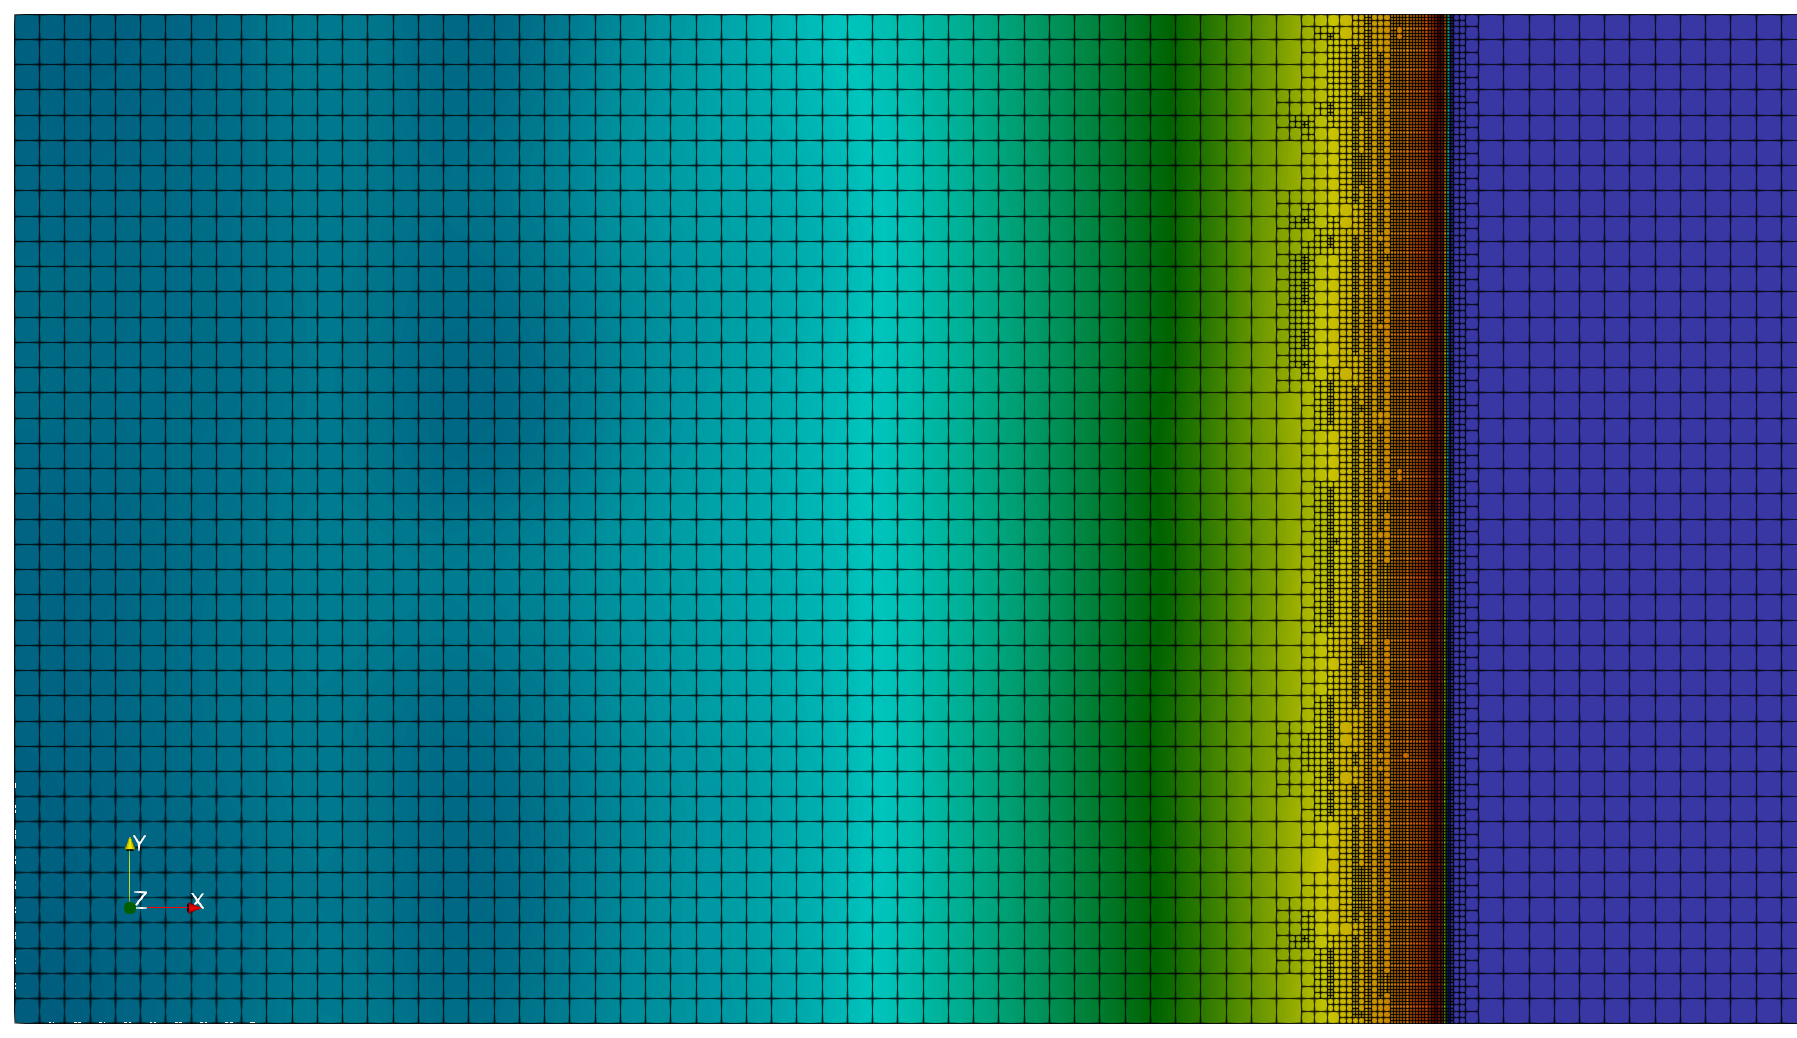
\includegraphics[width=0.69\textwidth]{../figs/amr_cells.png}
\caption{Three-level adaptive mesh refinement over a pressure field surface contour, with the detonation wave traveling from the -x wall to +x exit}
%\label{fig:examr}
\end{figure}
\end{frame}

\begin{frame}{Initial Meshing}
\begin{figure}[]
    \centering
    \begin{subfigure}[]{0.5\textwidth}
        \centering
        \includegraphics[width=\textwidth]{../figs/mesh/2Dmesh.png}
        \caption{Two-dimensional mesh}
    \end{subfigure}%
    \begin{subfigure}[]{0.5\textwidth}
        \centering
        \includegraphics[width=\textwidth]{../figs/mesh/3Dmesh.png}
        \caption{Three-dimensional mesh}
    \end{subfigure}
    %\caption{Static meshes used in OpenFOAM for detonation modeling, at an exaggerated unrefined resolution for example purposes}
    %\label{fig:meshcompare}
\end{figure}
\end{frame}

\begin{frame}[allowframebreaks]{Initial Detonation Attempts}
First testing \texttt{rhoReactingFoam}, methane-oxygen without nitrogen was used, with corner ignition to test shock reflection and exit 
\begin{figure}[]
\centering
\includegraphics[width=\textwidth]{../figs/cornerdet.png}
%\caption{Initial methane and oxygen detonation boundary condition test with corner detonation. Velocity magnitude is plotted here without scale to just check the solver and boundary conditions for modeling potential. Detonation was initiated in the lower left corner.}
%\label{fig:cornerdet}
\end{figure}%
Testing the detonation tube setup performed by Towery \textit{et. al.} \cite{towery1} was next, to be used as comparison. 

\newpage

\begin{columns}
\column{0.4\textwidth}
Different static mesh resolutions were tested with \texttt{rhoReactingFoam}, but noise and instability in the solution was seen.
\column{0.6\textwidth}
\begin{figure}[]
\centering
\includegraphics[width=\textwidth]{../figs/rhoReactingFoam.png}
%\caption{Noise and instability in solution and shock capturing problems using the \texttt{rhoReactingFoam} solver}
%\label{fig:rrf}
\end{figure}%
\end{columns}
\newpage

\begin{columns}
\column{0.6\textwidth}
\begin{figure}[]
\centering
\includegraphics[width=\linewidth]{../figs/shocktube.png} 
%\caption{Shock tube validated test case included with OpenFOAM compared to hybrid solver}
%\label{fig:sod}
\end{figure}%

\column{0.4\textwidth}
\begin{itemize}
\item turned towards the solvers utilizing central-upwind schemes of Kurganov and Tadmor \cite{kurganov1}
\item used the shock tube test to validate shock-capturing capability
\end{itemize}
\end{columns}
\end{frame}
